\chapter*{Methadology}
\addcontentsline{toc}{chapter}{Methadology}
\setcounter{chapter}{3}

\section{Data Collection}
The data collection process for this methodology involves several intricate steps, leveraging multiple data sources and employing various Python-based techniques 
to gather and process the required information. This section outlines the comprehensive approach taken to ensure the data is robust, reliable, and suitable for subsequent analysis and modeling.

\subsection{Financial Market Data Acquisition}
The first step in the data collection process involves obtaining financial market data from Yahoo Finance. This includes historical prices and volumes for a range of 
assets such as Bitcoin (BTC), Ethereum (ETH), Solana (SOL), gold, oil, Nvidia, the VIX, S\&P 500, and Dow Jones Industrial Average. The Python yfinance library is employed 
to access the Yahoo Finance API. This library provides an efficient way to retrieve historical price data, allowing us to gather data spanning the past five years. 
The collected data includes:

\begin{itemize}
    \item Daily closing prices
    \item Trading volumes
\end{itemize}

This data forms the foundation of the dataset, providing crucial information on market trends and volatility.

\subsection{Google Trends and Wikipedia Data}
To gauge public interest and sentiment, data from Google Trends and Wikipedia is incorporated. For Google Trends, the focus is on terms such 
as 'bitcoin', 'ethereum', 'solana', 'crypto', and 'blockchain'. This data is accessed using the pytrends library, which allows us to download historical 
search interest data for these terms. Similarly, Wikipedia page views for the same terms are collected using the Wikipedia API. The aggregation of this data
 involves summing the total page views and total search interest over the specified period. This provides a measure of the general public's engagement and interest in these topics.

\subsection{Reddit Sentiment Analysis}
Sentiment analysis is performed on Reddit posts related to Solana, sourced from three specific subreddits. The data is pulled using the Reddit API, focusing on the top 100 posts 
at the time of collection. The information retrieved includes:

\begin{itemize}
    \item Post titles
    \item Post descriptions (selftext)
    \item Number of upvotes
    \item Date posted
\end{itemize}

A sentiment analysis pipeline is implemented using the VADER (Valence Aware Dictionary and sEntiment Reasoner) sentiment analysis tool. The text data is 
preprocessed to remove noise, and sentiment scores are computed for each post. These scores are then aggregated by date, weighted by the number of upvotes, 
to calculate a mean weighted average sentiment for each day. This approach ensures that posts with higher engagement have a more significant impact on the sentiment measure.

\subsection{Total Value Locked (TVL)}
The total value locked (TVL) data for each cryptocurrency is obtained from Defi Lama. TVL represents the total capital held within a blockchain's DeFi ecosystem, 
providing insight into the level of trust and engagement from the community. This data is crucial for understanding the financial health and adoption of each cryptocurrency.

\subsection{Technical Indicators}
Technical indicators are derived from the historical price data obtained in the first step. A Python function is developed to calculate several key indicators, including:

\begin{itemize}
    \item Moving Average (MA)
    \item Exponential Moving Average (EMA)
    \item Stochastic Oscillators
    \item Relative Strength Index (RSI)
    \item Commodity Channel Index (CCI)
    \item Moving Average Convergence Divergence (MACD)
\end{itemize}

These indicators are used to create trend deterministic columns, where a value of 1 indicates a bullish signal and 0 indicates a bearish signal. 
These technical indicators are essential for understanding market trends and potential future movements.

\subsection{Data Merging and Preparation}
The final step in the data collection process involves merging all the collected data on the date field. This step integrates the financial market data, Google Trends and Wikipedia data,
 Reddit sentiment scores, TVL data, and technical indicators into a single cohesive dataset. The merged dataset is then ready for feature selection and modeling, ensuring that all relevant 
 information is available for comprehensive analysis.




\section{Feature Engineering}

\subsection{Technical Indicators:} Calculation of moving averages, RSI, MACD, Bollinger Bands, etc., using historical price and volume data.


\small
\begin{tabular}{|>{\raggedright\arraybackslash}m{2cm}|>{\raggedright\arraybackslash}m{10cm}|>{\raggedright\arraybackslash}m{5cm}|}
\hline
\textbf{Indicator} & \textbf{Formula} & \textbf{Trend Det. (1/0)} \\
\hline
10D MA & $MA = \frac{1}{10} \sum_{i=0}^{9} P_{t-i}$ & $1 \text{ if } P_t > MA, 0 \text{ else}$ \\
\hline
30D MA & $3MA = \frac{1}{30} \sum_{i=0}^{29} P_{t-i}$ & $1 \text{ if } P_t > 3MA, 0 \text{ else}$ \\
\hline
\%K & $\frac{P_t - LL}{HH - LL} \times 100$, $LL = \min(P_{t-9}, \ldots, P_t)$, $HH = \max(P_{t-9}, \ldots, P_t)$ & $1 \text{ if } \%K_t > \%K_{t-1}, 0 \text{ else}$ \\
\hline
\%D & $\frac{1}{3} \sum_{i=0}^{2} \%K_{t-i}$ & $1 \text{ if } \%D_t > \%D_{t-1}, 0 \text{ else}$ \\
\hline
RSI & $\Delta P_t = P_t - P_{t-1}$ \newline
$U_t = \frac{1}{14} \sum_{i=0}^{13} \max(\Delta P_{t-i}, 0)$ \newline
$D_t = \frac{1}{14} \sum_{i=0}^{13} \max(-\Delta P_{t-i}, 0)$ \newline
$RS = \frac{U_t}{D_t}$, $RSI = 100 - \frac{100}{1 + RS}$ & $\begin{cases}
-1 & RSI \geq 70 \text{ \& hold} \\
1 & RSI \leq 30 \\
0 & \text{else}
\end{cases}$ \newline
or \newline
$1 \text{ if } RSI \leq 30, 0 \text{ else}$ \\
\hline
Momentum & $P_t - P_{t-10}$ & $1 \text{ if } Mom > 1, 0 \text{ else}$ \\
\hline
MACD & $EMA_{12} = P_t \cdot \frac{2}{13} + EMA_{12,t-1} \cdot \frac{11}{13}$ \newline
$EMA_{26} = P_t \cdot \frac{2}{27} + EMA_{26,t-1} \cdot \frac{25}{27}$ \newline
$MACD = EMA_{12} - EMA_{26}$ \newline
$Signal = MACD_t \cdot \frac{2}{10} + Signal_{t-1} \cdot \frac{8}{10}$ & $1 \text{ if } MACD > MACD_{t-1}, 0 \text{ else}$ \\
\hline
CCI & $TP = \frac{H_t + L_t + P_t}{3}$ \newline
$SMA_{TP} = \frac{1}{20} \sum_{i=0}^{19} TP_{t-i}$ \newline
$MD = \frac{1}{20} \sum_{i=0}^{19} |TP_{t-i} - SMA_{TP}|$ \newline
$CCI = \frac{TP - SMA_{TP}}{0.015 \cdot MD}$ & $\begin{cases}
-1 & CCI \geq 100 \text{ \& hold} \\
1 & CCI \leq -100 \\
0 & \text{else}
\end{cases}$ \newline
or \newline
$1 \text{ if } CCI \leq -100, 0 \text{ else}$ \\
\hline
Bollinger & $SMA_{20} = \frac{1}{20} \sum_{i=0}^{19} P_{t-i}$ \newline
$STD_{20} = \sqrt{\frac{1}{20} \sum_{i=0}^{19} (P_{t-i} - SMA_{20})^2}$ \newline
$UB = SMA_{20} + 2 \cdot STD_{20}$ \newline
$LB = SMA_{20} - 2 \cdot STD_{20}$ & $\begin{cases}
-1 & P_t > UB \text{ \& hold} \\
1 & P_t < LB \\
0 & \text{else}
\end{cases}$ \newline
or \newline
$1 \text{ if } P_t < LB, 0 \text{ else}$ \\
\hline
ATR & $TR = \max(H_t, C_{t-1}) - \min(L_t, C_{t-1})$ \newline
$ATR = \frac{1}{14} \sum_{i=0}^{13} TR_{t-i}$ & $1 \text{ if } TR > ATR, 0 \text{ else}$ \\
\hline
\end{tabular}



\subsection{Reddit Sentiment Analysis:} Top 100 posts from Reddit communities for Bitcoin, Ethereum, and Solana. Sentiment analysis using VADER lexicon to derive bullish or bearish sentiment scores.

\subsubsection{Text Preprocessing}
The process began with the collection of Reddit posts, including both the titles and the text of each post. To ensure a comprehensive sentiment analysis, the titles and texts were combined into a single column for each post. The combined text was then preprocessed using the Natural Language Toolkit (nltk) in Python. This preprocessing involved several steps to clean the text and prepare it for analysis. First, the text was converted to lowercase to ensure uniformity. Punctuation and special characters were removed, and the text was tokenized into individual words. Common stop words such as "the," "and," and "is" were removed to reduce noise. Finally, lemmatization was performed to convert words to their base forms, such as converting "running" to "run." This preprocessing step ensured that the text was clean and ready for sentiment analysis.

\subsubsection{Sentiment Analysis with VADER}
For sentiment analysis, we utilized VADER (Valence Aware Dictionary and sEntiment Reasoner), a lexicon and rule-based tool specifically designed to handle sentiments expressed in social media contexts. VADER employs a lexicon-based approach, where each word in its predefined list has an associated sentiment score indicating whether it is positive, negative, or neutral. Additionally, VADER applies rules and heuristics to handle punctuation, capitalization, degree modifiers, and conjunctions. For example, exclamation marks increase the intensity of the sentiment, uppercase words indicate stronger sentiment, and words like "very" or "kind of" modify the intensity of the sentiment.

The combined title and text of each Reddit post were passed through VADER for sentiment analysis. VADER first split the text into individual sentences, then matched each word in the sentences against its lexicon to retrieve sentiment scores. The sentiment scores of words in a sentence were aggregated, with adjustments made for the rules and heuristics VADER applies. The sentence-level sentiments were then combined to produce the final sentiment scores for the entire post.

VADER provided four key sentiment scores for each post: positive, neutral, negative, and compound. The positive score represented the proportion of positive words in the text, the neutral score represented the proportion of neutral words, and the negative score represented the proportion of negative words. The compound score, a normalized measure that sums the overall sentiment of the text, ranged from -1 (extremely negative) to +1 (extremely positive). This comprehensive approach allowed us to capture the nuanced sentiment expressed in Reddit posts effectively.

\begin{figure}[h]
    \centering
    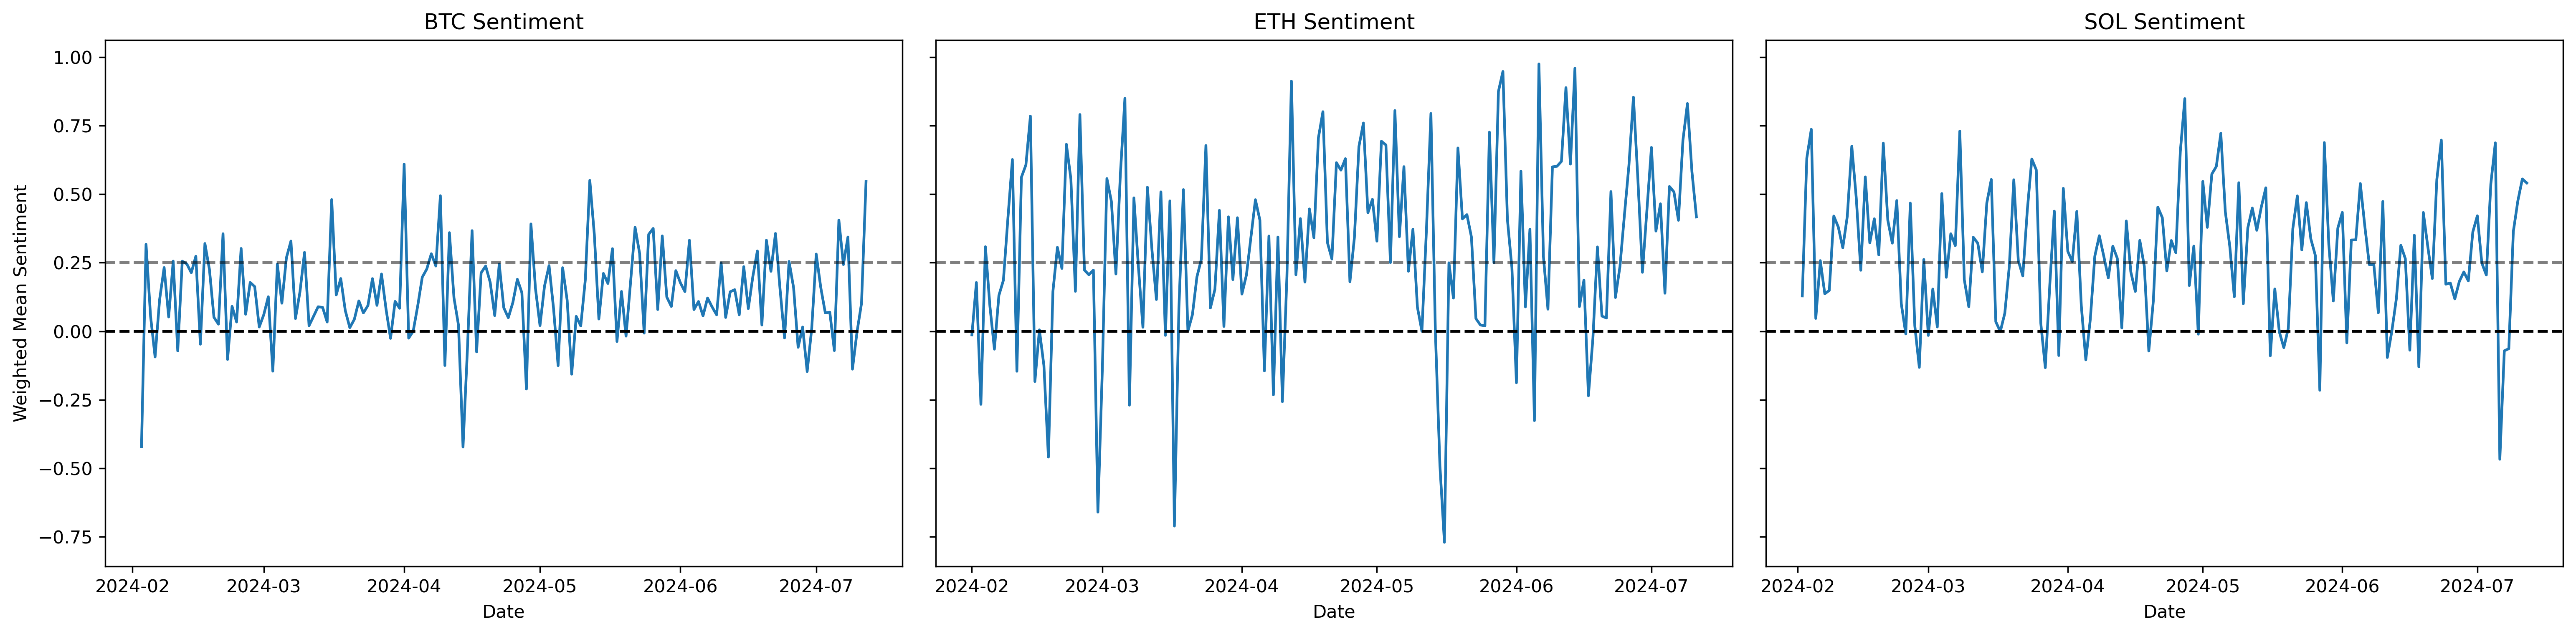
\includegraphics[width=190mm]{sentimentanalysis.png}
    \caption{Diagram showing Each Subreddits Sentiment}
    \label{fig:example-image}
\end{figure}


\subsection{Additional Features:} Inclusion of market indices data (S\&P 500, NVIDIA) as predictors.


\section{Machine Learning Models}
\subsection{Random Forest}
Random Forest is an ensemble learning method that operates by constructing a multitude of decision trees during training and outputting the mode of the classes (classification) or mean prediction (regression) of the individual trees. The principle behind Random Forest is to reduce the risk of overfitting by averaging multiple deep decision trees, trained on different parts of the same training set.

Mathematically, for a given input $\mathbf{x}$, the prediction of the $i$-th tree $h_i(\mathbf{x})$ in a random forest is:
\[
f(\mathbf{x}) = \frac{1}{N} \sum_{i=1}^N h_i(\mathbf{x})
\]
where $N$ is the number of trees in the forest.

Key parameters include:
\begin{itemize}
    \item Number of trees ($N$)
    \item Maximum depth of each tree
\end{itemize}

\subsection{Support Vector Classification (SVC)}

Support Vector Classification (SVC) aims to find the optimal hyperplane that maximizes the margin between the classes. This hyperplane is defined by the support vectors, which are the data points closest to the hyperplane.

The optimization problem for SVC can be written as:
\[
\min_{\mathbf{w}, b} \frac{1}{2} \|\mathbf{w}\|^2 \quad \text{subject to} \quad y_i (\mathbf{w} \cdot \mathbf{x}_i + b) \geq 1, \; \forall i
\]
where $\mathbf{w}$ is the weight vector, $b$ is the bias, $\mathbf{x}_i$ are the input vectors, and $y_i$ are the class labels.

Key parameters include:
\begin{itemize}
    \item Kernel type (linear, polynomial, radial basis function)
    \item Regularization parameter ($C$)
\end{itemize}

\subsection{Gradient Boosting Classification}

Gradient Boosting Classification is a sequential ensemble technique that builds models in a stage-wise manner. It optimizes for a loss function by adding weak learners to the model, typically decision trees.

The Prediction function for Gradient Boosting is:

\[ \hat{y} = F_M(x) = F_0(x) + \eta \sum_{m=1}^M h_m(x) \]

Where:
\begin{itemize}
\item \( \hat{y} \) is the predicted value.
\item \( F_0(x) \) is the initial prediction.
\item \( M \) is the total number of iterations (trees).
\item \( \eta \) is the learning rate.
\item  \( h_m(x) \) is the prediction from the \( m \)-th weak learner (tree).
\end{itemize}

Key parameters include:
\begin{itemize}
    \item Learning rate ($\eta$): The learning rate is a hyperparameter that controls the contribution of each weak learner (base model) to the final ensemble model. It scales the output of each weak learner before adding it to the accumulated model.
    \item Number of estimators: This parameter specifies the number of weak learners (usually decision trees) to be included in the ensemble. It defines how many iterations the boosting process will run.
    \item Maximum depth of each estimator: This parameter sets the maximum depth of the individual decision trees. It controls the complexity of the trees.
\end{itemize}

\subsection{Long Short-Term Memory (LSTM)}

Long Short-Term Memory (LSTM) networks are a type of recurrent neural network (RNN) capable of learning order dependence in sequence prediction problems. This subsection provides a detailed methodology of LSTM networks, explaining their working with equations and their application in the context of cryptocurrency analysis.

\subsubsection{LSTM Network Architecture}
An LSTM network consists of a series of LSTM cells, each containing three main components: a cell state, and three gates (input gate, forget gate, and output gate).

\paragraph{Cell State}
The cell state \(C_t\) acts as a memory that carries information across the sequence steps, enabling the network to maintain long-term dependencies.

\paragraph{Gates}
The gates regulate the flow of information into and out of the cell state. They are defined as follows:

\begin{itemize}
    \item \textbf{Forget Gate} (\(f_t\)): Decides what information to discard from the cell state.
    \item \textbf{Input Gate} (\(i_t\)): Decides which new information to add to the cell state.
    \item \textbf{Output Gate} (\(o_t\)): Decides what information to output based on the cell state.
\end{itemize}

\subsubsection{Equations of LSTM}
The mathematical formulation of the LSTM gates and cell state updates are given by the following equations:

\paragraph{Forget Gate}
\[
f_t = \sigma(W_f \cdot [h_{t-1}, x_t] + b_f)
\]

\paragraph{Input Gate}
\[
i_t = \sigma(W_i \cdot [h_{t-1}, x_t] + b_i)
\]
\[
\tilde{C}_t = \tanh(W_C \cdot [h_{t-1}, x_t] + b_C)
\]

\paragraph{Cell State Update}
\[
C_t = f_t * C_{t-1} + i_t * \tilde{C}_t
\]

\paragraph{Output Gate}
\[
o_t = \sigma(W_o \cdot [h_{t-1}, x_t] + b_o)
\]
\[
h_t = o_t * \tanh(C_t)
\]

Where:
\begin{itemize}
    \item \(x_t\) is the input at time step \(t\),
    \item \(h_{t-1}\) is the hidden state from the previous time step,
    \item \(\sigma\) is the sigmoid activation function,
    \item \(W_f, W_i, W_C, W_o\) are the weight matrices,
    \item \(b_f, b_i, b_C, b_o\) are the bias vectors.
\end{itemize}


\begin{figure}[h]
    \centering
    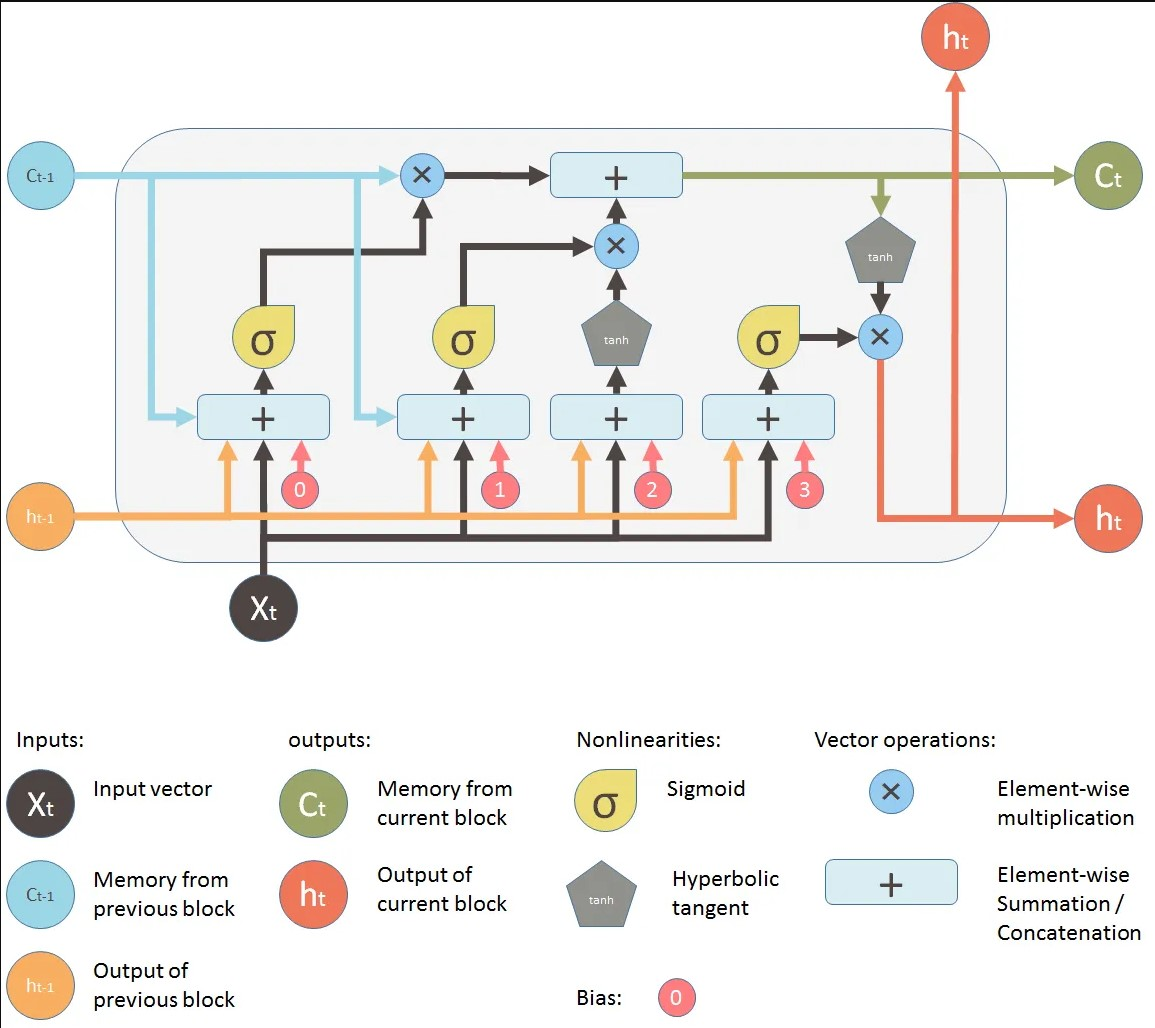
\includegraphics[width=160mm]{lstm.jpg}
    \caption{LSTM Diagram}
    \label{fig:example-image}
\end{figure}



\subsection{Hidden Markov Model (HMM)}

Hidden Markov Models (HMMs) are statistical models used for sequential data, where the system being modeled is assumed to be a Markov process with hidden states.

An HMM is defined by:
\begin{itemize}
    \item Number of hidden states ($N$)
    \item Transition probability matrix $A = \{a_{ij}\}$, where $a_{ij} = P(s_{t+1}=j | s_t=i)$
    \item Emission probability matrix $B = \{b_j(o_t)\}$, where $b_j(o_t) = P(o_t | s_t=j)$
\end{itemize}

The model works by estimating the sequence of hidden states given the observed data, typically using algorithms such as the Forward-Backward algorithm or Viterbi algorithm.

\[
P(O | \lambda) = \sum_{all \; paths} P(O, Q | \lambda)
\]

where $O$ is the sequence of observations, $Q$ is the sequence of hidden states, and $\lambda = (A, B, \pi)$ represents the model parameters.

An illustrative image showing the state transitions and observation emissions would help explain HMMs more effectively.


\section{Model Evaluation}
\begin{itemize}
    \item \textbf{Metrics:} Accuracy, precision, recall, F1-score, ROC-AUC for classification; MSE, MAE, R-squared for regression.
    \item \textbf{Cross-Validation:} K-fold cross-validation.
    \item \textbf{Model Comparison:} Performance metrics comparison to select the best model.
\end{itemize}
